\documentclass{article}
\usepackage[utf8]{inputenc}
\usepackage{graphicx}
\usepackage[section]{placeins}
\usepackage{float}
\usepackage{url}

\title{SocialIQA\_pt: A Translation of a Common-Sense Reasoning Dataset about Social Interactions}
\author{Fabio Grassiotto}
\date{30 June 2024}

\begin{document}

\maketitle

\begin{abstract}
    The objective of this work is to create a Portuguese language translation of
    the English dataset Social IQa, a benchmark of 38,000 multiple choice
    questions for the evaluation of emotional and social intelligence in a
    number of everyday situations. The approach taken here was to perform
    machine translation using popular models available at Hugging Face, rank
    translations using a GPT-driven evaluation (GEMBA) and select the best for
    our dataset.
\end{abstract}

\section{Introduction}

Common-Sense inteligence, defined usually as the human ability of applying
practical knowledge for decisions in everyday life, is still considered a
challenging task for AI systems. As it can be readily perceived when interacting
with chatbots, these systems lack the ability to, through intuition, reason
about common situations and events. Such reasoning requires background knowledge
about how the world works, incluind the rich nuanced interaction between people
in the social sphere \cite{choi2022curious, krause2023commonsense}.

Therefore, in artificial intelligence, the availability of datasets capable of
benchmarking this task is of utmost importance. Datasets such as Social IQa are
readily available in the english language, but we are not aware of any in
portuguese \cite{sap2019socialiqa}.

The portuguese language cannot be truly considered a low-resource language as
it is the case with some of the African and Asian languages, as there are
datasets already available in portuguese that have millions of tokens. There
are, however, certainly gaps that should be addressed \cite{ghafoor2021impact}.

One of these gaps lies in the availability of datasets that deal with common
sense-reasoning and in special datasets that adress social interactions.

This work is structured as follows:
\begin{itemize}
    \item Section 1 \textbf{(this section)}: Here we introduce the work and its
    motivation.
    \item Section 2 \textbf{Dataset}: We describe the SocialIQA original english
    language dataset.
    \item Section 3 \textbf{Methodology}: We describe the translation process
    and the evaluation system we employed.
    \item Section 4 \textbf{Results}: We describe the translated sets results
    and compare them in detail.
    \item Section 5 \textbf{Conclusion and Future Works}: We analyse the results
    we achieved and describe next steps to be taken.
\end{itemize}

\section{Dataset}
The Social Intelligence QA dataset was the first available resource upon its
publication for the measurement of social and emotional intelligence for AI
systems \cite{socialiqa}. The dataset, collected using a crowd-sourced framework,  is comprised
of around 38k multiple choice questions.

The Social IQa dataset is divided into 3 separate bases:
\begin{itemize}
    \item Development, with 1954 questions/answers.
    \item Training, with 33410 questions/answers.
    \item Test, with 2224 questions/answers.
\end{itemize}

Each row of the dataset consists of the following sequences of characters:

\begin{itemize}
    \item \textbf{Context} An observed context for a common situation.
    \item \textbf{Question} A question requiring reasoning about the social
    causes and effects of the observed situation.
    \item \textbf{Answer A, Answer B, Answer C} Multiple choices for answers.
    Besides one correct answer, the other two are collected from four negative
    options that were handwritten to be similar to the correct answers in terms
    of topic, length, and style but are subtly incorrect.
    \item \textbf{Correct} The expected correct answer to the question as
    determied by human peers.
\end{itemize}

An example of the types of questions and choices can be seen below on Table
\ref{table:SocialIQa}. These are the first few rows from the development section
of the development section of the dataset.
\begin{table}[!ht]
    \makebox[\textwidth][c]{
        \begin{tabular}{|p{0.9in}|p{0.9in}|p{0.9in}|p{0.9in}|p{0.9in}|p{0.9in}|}\hline
        \textbf{Context}                                                                                                                              & \textbf{Question}                                & \textbf{Answer A}                                                   & \textbf{Answer B}                                                  & \textbf{Answer C}                                            & \textbf{Correct} \\\hline
        Tracy didn't go home that evening and resisted Riley's attacks.                                                                      & What does Tracy need to do before this? & make a new plan                                           & Go home and see Riley                                    & Find somewhere to go                               & C       \\\hline
        Sydney walked past a homeless woman asking for change but did not have any money they could give to her. Sydney felt bad afterwards. & How would you describe Sydney?          & sympathetic                                               & like a person who was unable to help                     & incredulous                                        & A       \\\hline
        Sasha protected the patients' rights by making new laws regarding cancer drug trials.                                                & What will patients want to do next?     & write new laws                                            & get petitions signed                                     & live longer                                        & B       \\\hline
        Jordan was in charge of taking the food on the camping trip and left all the food at home.                                           & How would Jordan feel afterwards?       & horrible that he let his friends down on the camping trip & happy that he doesn't need to do the cooking on the trip & very proud and accomplished about the camping trip & A       \\\hline
        \end{tabular}}
        \caption{Example rows from the SocialIQa English dataset.}\label{table:SocialIQa}
\end{table} 

\section{Methodology} 

Our methodology consisted of two macro-phases, (1) machine translation using
neural network models and (2) comparative evaluation of the translations we
obtained using a large language model. After these macro-phases the best ranked
translation for each row of the dataset was selected for our final dataset.

\subsection{Machine Translation}
\label{subsec:machine-translation}

Three machine translation models were selected based on their popularity (amount
of downloads) from the Hugging Face website for this phase. The descriptions
below are taken verbatim from the model cards on the site.

\subsubsection{Helsinki-NLP/opus-mt-tc-big-en-pt}

\begin{quote}
This model is part of the OPUS-MT project \cite{tiedemann2020opus}, an effort to
make neural machine translation models widely available and accessible for many
languages in the world. All models are originally trained using the amazing
framework of Marian NMT, an efficient NMT implementation written in pure C++.
The models have been converted to pyTorch using the transformers library by
huggingface. Training data is taken from OPUS and training pipelines use the
procedures of OPUS-MT-train.
\end{quote}

\subsubsection{unicamp-dl/translation-en-pt-t5}

\begin{quote}
This repository brings an implementation of T5 for translation in PT-EN and
EN-PT tasks using a modest hardware setup. We propose some changes in
tokenizator and post-processing that improves the result and used a Portuguese
pretrained model for the translation \cite{lopes2020lite}.
\end{quote}

\subsubsection{facebook/nllb-200-distilled-1.3B}

\begin{quote}
NLLB-200 is a machine translation model primarily intended for research in
machine translation, especially for low-resource languages. It allows for
single sentence translation among 200 languages \cite{costa2022no}.
\end{quote}

\subsection{Translation Evaluation}
\label{subsec:translation-evaluation}

There are a number of alternatives for evaluating translations
\cite{lee2023survey}. Evaluations using large language models have been producing
results closer to human evaluation and therefore we selected this method for
this work.

The three translations were thus compared using the evaluation metric
GEMBA - GPT Estimation Metric Based Assessment \cite{kocmi2023large} using
GPT3.5-turbo. To use the metric, the prompt was modified to not use human
reference in the evaluation and to evaluate the translations of the three models
of this work simultaneously.

The modified GEMBA prompt used to query GPT3.5 turbo was:

\begin{verbatim}
You are a helpful evaluator of the quality of translations.
Score the following translations from English to Portuguese on a
continuous scale from 0 to 100, where a score of zero means
"no meaning preserved" and score of one hundred means "perfect
meaning and grammar".

En: source_seg
Pt 1: target_seg1
Pt 2: target_seg2
Pt 3: target_seg3
Reply with only the number scores of your evaluation, in a 
python list:
\end{verbatim}

Where \emph{source\_seg} is the original language group of sentences, and
\emph{target\_seg*} are the proposed translations from each model. GPT-3.5-turbo
replies to this prompt with a Python-style list with the rankings e.g. [80, 85,
100].

\subsection{Workflow}
Our workflow consisted of the five steps described in Figure
\ref{fig:diagram} below. All steps are executed using Python notebook files
available at.

\begin{itemize}
    \item \textbf{Step I: English dataset conversion} In this step, the original
    english dataset was converted from JSON format into a temporary 
    comma-delimited file format for easier processing. The conversion was
    performed on file read\_dataset\_en.ipynb.
    \item \textbf{Step II: Machine Translation} In this step, the original
    dataset, available in three separate files for the development, training and
    testing sets, was translated to the portuguese language using the three
    distinct models described in \ref{subsec:machine-translation}. The
    implementations are on files translator\_marian.ipynb, translator\_t5.ipynb
    and translator\_nllb.ipynb.
    \item \textbf{Step III: Translation Evaluation} In this step, translations were evaluated
    using the evaluation metric GEMBA as described in \ref{subsec:translation-evaluation}
    \item \textbf{Step IV: Translation selection and ranking} The highest ranked translation set
    was selected based on the metric described above and used in the dataset.
    The implementation for steps III and IV is executed on files
    evaluator\_gemba\_dev.ipynb, evaluator\_gemba\_train.ipynb and
    evaluator\_gemba\_tsyt.ipynb respectively for the development, training and
    test sets.
    \item \textbf{Step V: Portuguese Dataset publishing}  In this step, the
    comma-delimited file with the final translation contents was converted to
    JSONL format for publishing. The conversion was performed on file 
    publish\_dataset\_pt.ipynb.
\end{itemize}
 
\begin{figure}[htbp]
    \centering
    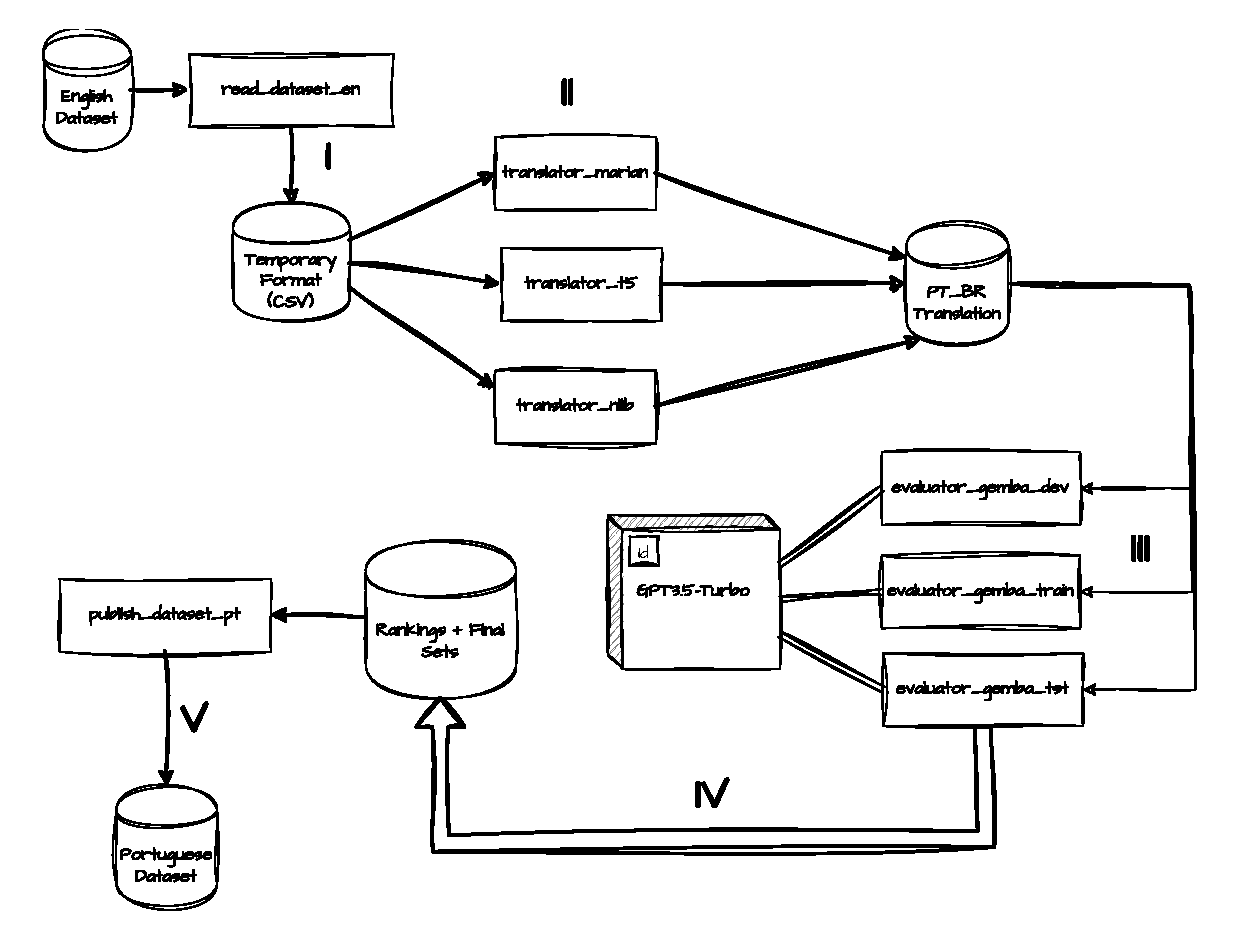
\includegraphics[width=0.8\textwidth]{drawio/translation.drawio.pdf}
    \caption{\label{fig:diagram}Translation process including machine
    translation and GPT-based evaluation to select the best possible
    translation.}
\end{figure}

\section{Results}

We have compared the results of the translations using the GEMBA method as can be seen below.

\subsection{Selected Translations per Model}

As can be seen on Figure \ref{fig:pie}, the model we selected most of our
translations was the NLLB-1.3b from Meta. We believe this is due to the fact
that the strengths of this model lie on the translations of short sentences. It
is worthy noting that this is the largest model of the group.

\begin{figure}[htbp]
    \centering
    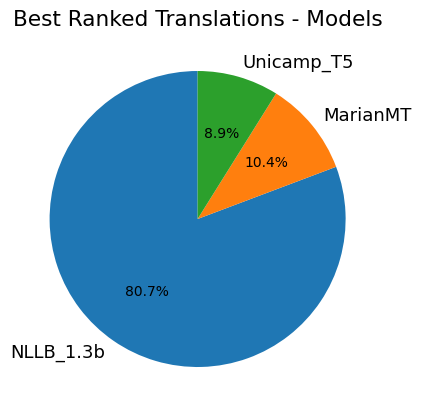
\includegraphics[width=0.4\textwidth]{figures/pie-chart.png}
    \caption{\label{fig:pie}Selected Translations per Model.}
\end{figure}
\FloatBarrier

\subsection{Kernel Density Estimates}

On figure \ref{fig:kde} we plot the Kernel Density Estimates for the
distribution of the ratings for each model. We note that NLLB-1.3b has the most
evaluations towards largest evaluations, while the T5 model has a more flat
distribution.

\begin{figure}[htbp]
    \centering
    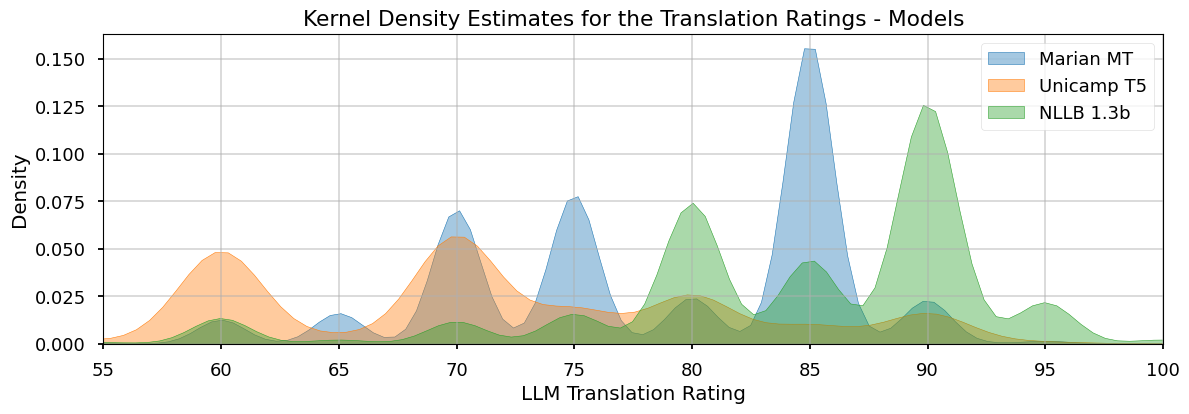
\includegraphics[width=0.9\textwidth]{figures/kde.png}
    \caption{\label{fig:kde}KDE distributions per Model.}
\end{figure}
\FloatBarrier

\subsection{Ratings per Sequence Length}

We proceed then to evaluate the impact of sequence length on the translation
quality in Figure \ref{fig:line-chart}. We did not notice appreciable difference
among the models we used.

\begin{figure}[htpb]
    \centering
    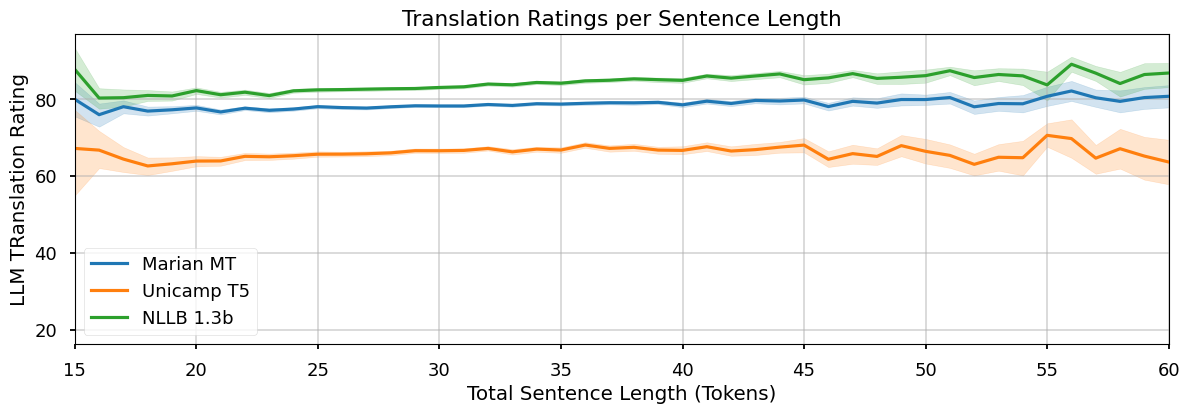
\includegraphics[width=0.9\textwidth]{figures/line-chart.png}
    \caption{\label{fig:line-chart}Rating per Sequence Length per Model.}
\end{figure}

\section{Conclusion and Future Work}

The portuguese language dataset was published at Hugging face at \cite{socialiqa_pt}. 

We should note here some of the advantages and difficulties we found during the
conduction of this work. First, machine translation models with low hardware
requirements were necessary enablers for this work. All the translations were
performed locally with a consumer-grade graphics card with 16Gb of video RAM.
The usage of the GPT-3.5-turbo API in 2024 for a comparatively large dataset
(38k lines) was only feasible due the low cost. For the translation evaluation,
over 50 thousand requests and 16 million tokens were sent using the OpenAI API
at an estimated total cost of less than US\$ 10. It is worth noting, however,
that OpenAI API speed was quite slow requiring over 50 hours for the whole
process.

As future work, a through evaluation of the resulting dataset will be required
to remove incorrections from the translation process. We note also that due to
the fact that common-sense reasoning being very sensitive to cultural
differences, a review of the dataset by portuguese language speakers would be
extremely valid for improving the quality of the translation results.

\bibliographystyle{plain}
\bibliography{main.bib}

\end{document}
